% Provenance (never printed): see sources/outline_sources.md (Year 3:
% facies analysis, depositional models, Walther's law, well logs). Brief:
% sources/book5/BRIEFS.md, ch. 17. Curves from figdata/bachelor-3/well_logs.py
% (unit tops from figdata/shared/region.py). Exercise and problem values in
% the Book 5 scratch calculator calc/ch17.py. The well Varden-2, its logs and
% the channel architecture of its sandstone are invented.
\chapter{النماذج السحنية}\label{ch:b3:facies-models}

اللبّ المستخرج من بئر عمقها كيلومتر واحد: متر من رمل خشن ذي طبقات متصالبة
يرقد على قاعدة حادة، ويتناعم نحو الأعلى ليصير غرينًا تظهر فيه آثار الجذور،
ثم رمل آخر على قاعدة حادة أخرى. يقرأ الجيولوجي نهرًا
كان يتلوّى عبر سهله، رغم أنّه لا يجري هناك نهر الآن. ويستند التفسير إلى أداتين:
مجموعة من النماذج، كلّ منها خلاصة لأمثلة كثيرة حديثة وقديمة لبيئة واحدة،
وقانون يحوّل التعاقب الرأسي للطبقات
إلى خريطة للبيئات المتجاورة.

\begin{recall}
السحنات الرسوبية، والبيئة الترسيبية، والأشكال القاعية، والتطبّق المتصالب،
والدلتات بأنواعها الثلاثة، وتيارات العكارة، والعكرات، والطبقات المتدرّجة
واردة في مجلد السنة الأولى، في فصله عن الرواسب الفتاتية وبيئاتها،
والمصنع الكربوناتي والشعب المرجانية والمنصّات الكربوناتية في فصله
عن الرواسب الكربوناتية والسيليسية والتبخّرية، وسجلّ ثقب الحفر
وترابط السجلّات في فصله عن المقاطع العرضية. والمسامية والنفاذية
واردتان في كتب المدرسة. والمتتاليات الفرعية وسطوح الغمر ومسالك الأنظمة
واردة في الفصل~\ref{ch:b3:sequence-stratigraphy}. أما الأمواج في المياه العميقة،
التي تتلاشى حركتها مع العمق، فواردة في كتب الفيزياء.
\end{recall}

\section{السحنات والتعاقبات وقانون فالتر}\label{sec:b3:facies-models:walther}

تُوصف السحنة الرسوبية مما يُرى في اللبّ أو في
جرف صخري: حجم الحبيبات، ودرجة الفرز، والبنى، والأحافير، واللون. ونادرًا ما تكون السحنة الواحدة
تشخيصية، فالرمال المتصالبة تتكوّن في الأنهار وعلى الشواطئ وفي القنوات المدّية
وفي الصحارى. ما يعيّن البيئة هو الرفقة التي تصاحب السحنة،
وترتيب السحنات في تعاقبها بعضها إثر بعض.

\begin{definition}[تجمّع السحنات وتعاقب السحنات]\label{def:b3:facies-models:association}
\emph{تجمّع السحنات}\index{تجمّع السحنات} هو مجموعة من السحنات
تتواجد معًا وتُرسَّب في بيئة واحدة، مثل رمل القناة،
وغرين الجسر الطبيعي، وطين السهل الفيضي المحمَّل بالجذور.
و\emph{تعاقب السحنات}\index{تعاقب السحنات} تتابع رأسي للسحنات تتغيّر فيه خاصية ما تدريجيًا نحو الأعلى؛ وفي
\emph{التعاقب المتناعم نحو الأعلى}\index{التعاقب المتناعم نحو الأعلى} يتناقص حجم الحبيبات نحو الأعلى،
وفي \emph{التعاقب المتخاشن نحو الأعلى}\index{التعاقب المتخاشن نحو الأعلى}
يزداد
حجم الحبيبات نحو الأعلى.
\end{definition}

\begin{definition}[نموذج السحنة]\label{def:b3:facies-models:model}
\emph{نموذج السحنة}\index{نموذج السحنة} خلاصة عامة لبيئة ترسيبية،
مستخلصة من أمثلة حديثة وقديمة كثيرة: السحنات التي تنتجها،
وهندستها وعلاقاتها الجانبية والتعاقبات التي تبنيها.
ويُستعمل معيارًا لمقارنة مثال جديد به، ودليلًا
للمشاهدة اللاحقة، ومتنبِّئًا في الحالات الجديدة، وأساسًا
لتفسير البيئة.
\end{definition}

الجسر الذي يصل الجانبي بالرأسي هو قانون. والبيئات المتجاورة
ترقد جنبًا إلى جنب في أيّ لحظة: الشاطئ بجوار \omterm{def:b3:facies-models:shoreface}{الوجه الشاطئي}،
\omterm{def:b3:facies-models:shoreface}{والوجه الشاطئي} بجوار الطين البحري المفتوح. وعندما يتحرّك خط الشاطئ،
تأتي كلّ بيئة لترقد فوق جارتها.

\begin{theorem}[قانون فالتر]\label{thm:b3:facies-models:walther}
في تعاقب متوافق، دون انقطاع معتبر في الترسيب أو
سطح تعرية، فإنّ السحنات الراقدة مباشرة بعضها فوق بعض رُسّبت
في بيئات كانت متجاورة في ذلك الزمن.
\end{theorem}

\begin{proof}
لنتأمّل نطاقات من البيئات، كلّ منها شريط موازٍ لخط الشاطئ، تنتقل معًا
عبر الحوض أثناء هبوط القاع أو ارتفاع مستوى سطح البحر.
وعند مكان ثابت تمرّ النطاقات واحدًا تلو الآخر، بالترتيب الذي تقع به جنبًا إلى جنب،
ويترك كلّ نطاق رسوبه فوق رسوب النطاق الذي سبقه.
فإذا كان الترسيب مستمرًّا، فإنّ الترتيب الرأسي للرسوبات
هو إذن الترتيب الجانبي للنطاقات.
ويقطع الانقطاع أو سطح التعرية هذا الاستدلال:
فالنطاقات التي مرّت خلال الفجوة لم تترك شيئًا، أو أُزيلت رسوباتها،
فتتلامس سحنات من بيئات غير متجاورة.
\end{proof}

\begin{omfigure}
\begin{tikzpicture}[font=\scriptsize, x=1cm, y=1cm]
% environments side by side, with a shoreline that moves seaward
\fill[yellow!35!brown!25] (0,0) rectangle (3,0.5);
\fill[yellow!30] (3,0) rectangle (4.4,0.5);
\fill[yellow!50!orange!30] (4.4,0) rectangle (6.4,0.5);
\fill[black!20] (6.4,0) rectangle (9,0.5);
\draw (0,0) rectangle (9,0.5);
\foreach \x in {3,4.4,6.4} {\draw (\x,0) -- (\x,0.5);}
\node at (1.5,0.25) {السهل الساحلي};
\node at (3.7,0.25) {الشاطئ};
\node at (5.4,0.25) {الوجه الشاطئي};
\node at (7.7,0.25) {الطين البحري المفتوح};
\draw[->, thick] (3.2,0.9) -- (5.2,0.9) node[right] {تتحرّك النطاقات نحو البحر};
\node[anchor=south] at (4.5,1.2) {\foreignlanguage{arabic}{(أ) بيئات متجاورة}};
% vertical succession at a place
\begin{scope}[xshift=11cm, yshift=-1.2cm]
\fill[black!20] (0,0) rectangle (0.9,0.8);
\fill[yellow!50!orange!30] (0,0.8) -- (0.9,0.8) -- (1.3,1.8) -- (0,1.8) -- cycle;
\fill[yellow!30] (0,1.8) rectangle (1.4,2.4);
\fill[yellow!35!brown!25] (0,2.4) rectangle (1.0,3.1);
\draw (0,0) -- (0.9,0) -- (0.9,0.8) -- (1.3,1.8) -- (1.4,1.8) -- (1.4,2.4) -- (1.0,2.4) -- (1.0,3.1) -- (0,3.1) -- cycle;
\node[anchor=west] at (1.6,0.4) {الطين البحري المفتوح};
\node[anchor=west] at (1.6,1.3) {رمل الوجه الشاطئي};
\node[anchor=west] at (1.6,2.1) {الشاطئ};
\node[anchor=west] at (1.6,2.75) {السهل الساحلي};
\draw[->] (-0.3,0) -- (-0.3,3.1) node[above] {أعلى};
\node[anchor=north, align=center] at (0.9,-0.1) {\foreignlanguage{arabic}{(ب) التعاقب}\\ عند مكان واحد};
\end{scope}
\end{tikzpicture}

\par\smallskip{\small قانون والتر. (أ) تتجاور البيئات على امتداد
مقطع؛ (ب) مع انتقال الأحزمة نحو البحر، يتلقّى موقعٌ واحد الطينَ البحري المفتوح،
ثم رمل \omterm{def:b3:facies-models:shoreface}{الوجه الشاطئي} ورمل الشاطئ ورواسب السهل الساحلي: التعاقبَ
المتخاشنَ نحو الأعلى وفق ترتيب الأحزمة (يدلّ عرض السجلّ
على حبيبات أخشن).}\label{fig:b3:facies-models:walther}
\end{omfigure}

يعمل القانون في الاتجاهين. يُراكِم الانحسارُ الأحزمةَ وفق ترتيبها نحو البحر
نحو الأعلى، ويُراكِم التجاوزُ البحري الأحزمةَ بالترتيب المعكوس؛ والتعاقبُ الرأسي المقروء في
لبٍّ يعطي خريطة البيئات المجاورة في ذلك الزمن. ويخفق القانون
تحديدًا حيث يضع الفصل~\ref{ch:b3:sequence-stratigraphy} أسطحه الرئيسية:
عبر \omterm{def:b3:sequence-stratigraphy:sequence}{حدّ المتتالية}، حيث يجلب التعرّض والتعرية رمل النهر فوق
طين الرصيف، وعبر \omterm{def:b3:sequence-stratigraphy:parasequence}{سطح الغمر}، حيث يقع الطين البحري المفتوح مباشرة على
السهل الساحلي.

\section{الأنهار}\label{sec:b3:facies-models:rivers}

\begin{definition}[النهر المضفور والنهر المتعرّج]\label{def:b3:facies-models:rivers}
يجري \emph{النهر المضفور}\index{النهر المضفور} في عدّة قنوات ضحلة تتفرّع وتلتقي من جديد حول الحواجز،
تتفرّع وتلتقي من جديد حول الحواجز، على سهل شديد الانحدار تكثر فيه الحمولة الخشنة
وتصريف متغيّر. ويجري \emph{النهر المتعرّج}\index{النهر المتعرّج}
في قناة واحدة متعرّجة على سهل أقلّ انحدارًا، ويحمل المزيد
من الرواسب الناعمة؛ ويهاجر بتعرية الضفة الخارجية لكلّ انعطاف،
وترسيبِ المواد على الضفة الداخلية. والرسوب على الضفة الداخلية هو \emph{الحاجز
النقطي}\index{الحاجز النقطي}. \emph{انقلاب المجرى}\index{انقلاب المجرى} هو هجرُ
القناةَ لمسار جديد عبر السهل الفيضي، وغالبًا بعد أن يخترق فيضانٌ
السدّ الطبيعي.
\end{definition}

ينمو \omterm{def:b3:facies-models:rivers}{الحاجز النقطي} جانبيًا مع هجرة الانعطاف، فيسجّل في أيّ موضع
المقطعَ العرضي للقناة من الأسفل إلى الأعلى: رواسبَ متبقيةً من الفتات الأخشن
على قاعدة تعرّيّة، ورملًا متطبّقًا متقاطعًا من كثبان القناة العميقة،
ورملًا أدقّ مع التموّج الصغير من القمّة الضحلة للحاجز، ثم
الغرين والطين من السهل الفيضي مع الجذور والتربة. ووفق قانون والتر يكون هذا
التعاقبُ المتناعم نحو الأعلى، وهو بسماكة بضعة أمتار، يساوي
عمقَ القناة. ويخلّف \omterm{def:b3:facies-models:rivers}{النهر المضفور} طبقاتٍ متراكبة من الرمل المتقاطع
والحصى مع قليل من الطين، لا يتغيّر حجم حبيباتها تقريبًا نحو الأعلى؛ ويُنقل ناعمُها
بعيدًا. ويحرّك انقلابُ المجرى حزامَ القناة عبر السهل، بحيث
تتراكم أجسام القنوات عشوائيًا بين طين السهل الفيضي، مفصولةً بقواعد
تعرّيّة حادّة.

\begin{omfigure}
\begin{tikzpicture}[font=\scriptsize, x=1cm, y=1cm]
% (a) braided plan
\begin{scope}
\fill[yellow!35!brown!20] (0,0) rectangle (4.6,2.4);
\draw[omDef!60, line width=1.6pt] (0,1.2) .. controls (0.8,1.6) and (1.4,0.6) .. (2.3,1.0) .. controls (3.0,1.3) and (3.6,0.7) .. (4.6,1.0);
\draw[omDef!60, line width=1.6pt] (0,1.2) .. controls (0.8,0.8) and (1.6,1.9) .. (2.4,1.6) .. controls (3.2,1.3) and (3.8,1.9) .. (4.6,1.6);
\draw[omDef!60, line width=1.2pt] (1.2,1.25) .. controls (1.8,1.5) and (2.6,1.2) .. (3.3,1.35);
\fill[yellow!45] (1.5,1.15) ellipse (0.35 and 0.12);
\fill[yellow!45] (3.0,1.25) ellipse (0.4 and 0.12);
\node[anchor=south] at (2.3,2.45) {\foreignlanguage{arabic}{(أ) مضفور}};
\end{scope}
% (b) meandering plan
\begin{scope}[xshift=5.4cm]
\fill[green!30!black!12] (0,0) rectangle (4.6,2.4);
\draw[omDef!60, line width=2pt] (0,1.2) .. controls (0.6,2.2) and (1.4,2.2) .. (1.6,1.2) .. controls (1.8,0.2) and (2.8,0.2) .. (3.0,1.2) .. controls (3.2,2.2) and (4.0,2.2) .. (4.6,1.2);
\fill[yellow!45] (0.8,1.45) ellipse (0.3 and 0.2);
\fill[yellow!45] (2.3,0.95) ellipse (0.3 and 0.2);
\fill[yellow!45] (3.8,1.45) ellipse (0.3 and 0.2);
\node at (2.3,0.95) {pb};
\draw[omDef!40, line width=1pt, densely dashed] (0.4,0.2) .. controls (1.0,0.7) and (1.6,0.4) .. (2.0,0.1);
\node[anchor=west, font=\tiny] at (2.6,2.15) {السهل الفيضي};
\node[anchor=south] at (2.3,2.45) {\foreignlanguage{arabic}{(ب) متعرّج}};
\end{scope}
% logs
\begin{scope}[xshift=10.8cm]
\fill[yellow!45] (0,0) -- (1.2,0) -- (1.2,2.0) -- (0,2.0) -- cycle;
\draw (0,0) -- (1.2,0) -- (1.15,0.6) -- (1.2,0.65) -- (1.1,1.3) -- (1.2,1.35) -- (1.15,2.0) -- (0,2.0) -- cycle;
\node[anchor=north] at (0.6,-0.05) {مضفور};
\end{scope}
\begin{scope}[xshift=12.6cm]
\fill[yellow!45] (0,0) -- (1.2,0) -- (1.1,0.9) -- (0.45,1.6) -- (0,1.6) -- cycle;
\fill[green!30!black!15] (0,1.6) rectangle (0.3,2.2);
\draw (0,0) -- (1.2,0) -- (1.1,0.9) -- (0.45,1.6) -- (0.3,1.6) -- (0.3,2.2) -- (0,2.2) -- cycle;
\draw[decorate, decoration={snake, amplitude=0.4mm, segment length=1.5mm}] (0,0) -- (1.2,0);
\node[anchor=north] at (0.6,-0.05) {الحاجز النقطي};
\node[anchor=west, font=\tiny] at (0.35,1.9) {جذور};
\end{scope}
\end{tikzpicture}

\par\smallskip{\small (أ) \omterm{def:b3:facies-models:rivers}{النهر المضفور}: عدّة قنوات حول حواجز من الرمل
والحصى. (ب) \omterm{def:b3:facies-models:rivers}{النهر المتعرّج}: قناة واحدة متعرّجة، والحواجز النقطية (pb)
على الضفاف الداخلية، ومجرى مهجور (متقطّع) تركه \omterm{def:b3:facies-models:rivers}{انقلاب المجرى}. يسارًا:
سجلّات أحجام الحبيبات للرواسب (يعني العرض حبيبات أخشن): صفائح رملية متراكمة
قليلة التغيّر نحو الأعلى للنهر المضفور، \omterm{def:b3:facies-models:association}{والتعاقب المتناعم نحو الأعلى} ذو القاعدة
الحادّة يعلوه طين السهل الفيضي ذو الجذور، بالنسبة إلى \omterm{def:b3:facies-models:rivers}{الحاجز
النقطي}.}\label{fig:b3:facies-models:rivers}
\end{omfigure}

\section{خطوط الشاطئ والدلتات والأرصفة}\label{sec:b3:facies-models:shelves}

الدلتات في مجلد السنة الأولى، التي تسيطر عليها الأنهار أو الأمواج أو المدّ، وكلّها
تنمو نحو البحر بالآلية نفسها: يُرسّب المصبّ حمولته حيث
يتباطأ التيار، وتتقدّم جبهة الدلتا فوق طين الدلتا الأمامي الخاص بها.
يُخلّف \omterm{def:b3:facies-models:shoreface}{الوجه الشاطئي} أو جبهة الدلتا المتقدّمة، وفق قانون والتر، \omterm{def:b3:facies-models:association}{التعاقب
المتخاشن نحو الأعلى}: الطين البحري المفتوح، والطين المتداخل مع رمل العواصف،
ورمل \omterm{def:b3:facies-models:shoreface}{الوجه الشاطئي}، ثم الشاطئ. وكلّ متتالية فرعية من الفصل السابق هي
تعاقبٌ من هذا النوع.

\begin{definition}[الوجه الشاطئي وقواعد الأمواج]\label{def:b3:facies-models:shoreface}
\emph{الوجه الشاطئي}\index{الوجه الشاطئي} هو المنطقة المائلة الواقعة نحو البحر من
الشاطئ التي تعيد فيها الأمواج باستمرار تشكيل قاع البحر. وقاعدته هي
\emph{قاعدة أمواج الطقس الهادئ}\index{قاعدة أمواج الطقس الهادئ}، وهي العمق الذي تحته
لا تحرّك الأمواج الاعتيادية الرواسب القاعية بعد الآن. و\emph{قاعدة أمواج
العواصف}\index{قاعدة أمواج العواصف} هي الحدّ الأعمق الذي تبلغه أمواج العواصف؛
وبين الاثنين يترسّب الطين في الطقس الهادئ، ثم يُعاد تشكيله طبقاتٍ رملية
خلال العواصف. وتحت قاعدة أمواج العواصف يبقى القاعُ غيرَ مضطرب بالأمواج.
\end{definition}

\begin{omfigure}
\begin{tikzpicture}[font=\scriptsize, x=1cm, y=1.6cm]
\fill[omSea!60] (0,2.2) -- (13,2.2) -- (13,0.2) -- (5.5,0.9) -- (2.0,1.9) -- (0.6,2.2) -- cycle;
\fill[yellow!40] (0,2.4) -- (0.6,2.2) -- (2.0,1.9) -- (5.5,0.9) -- (5.5,0.0) -- (0,0.0) -- cycle;
\fill[black!18] (5.5,0.9) -- (13,0.2) -- (13,0) -- (5.5,0) -- cycle;
\draw[thick] (0,2.4) -- (0.6,2.2) -- (2.0,1.9) -- (5.5,0.9) -- (13,0.2);
\draw[omDef] (0,2.2) -- (13,2.2);
\draw[omDef, densely dashed] (1.6,1.97) -- (13,1.97);
\draw[omDef, densely dashed] (5.5,0.9) -- (13,0.9);
\node[omDef, anchor=north west] at (9.3,1.95) {قاعدة أمواج الطقس الهادئ};
\node[omDef, anchor=north west] at (9.3,0.88) {قاعدة أمواج العواصف};
\node[anchor=south] at (0.5,2.42) {الشاطئ};
\node at (1.8,1.35) {الوجه الشاطئي};
\node at (4.3,0.45) {الانتقال نحو عرض البحر};
\node at (9.0,0.15) {طين عرض البحر};
\node[align=center] at (7.4,1.45) {\foreignlanguage{arabic}{طبقات رملية للعواصف،}\\ التطبّق المتقاطع الرابي};
\end{tikzpicture}

\par\smallskip{\small مقطع تخطيطي لخط شاطئ تسيطر عليه الأمواج (تخطيطي، والمقياس الرأسي
مكبَّر بدرجة كبيرة). فوق \omterm{def:b3:facies-models:shoreface}{قاعدة أمواج الطقس الهادئ} يُعاد تشكيل رمل \omterm{def:b3:facies-models:shoreface}{الوجه الشاطئي}
يوميًا؛ وبين قاعدتي الأمواج يتناوب الطين مع
طبقات رملية مترسّبة بفعل العواصف؛ وتحت \omterm{def:b3:facies-models:shoreface}{قاعدة أمواج العواصف}
يتراكم الطين.}\label{fig:b3:facies-models:shoreface}
\end{omfigure}

تتلاشى الحركة المدارية للموجة في المياه العميقة وفق $e^{-2\pi z/\lambda}$
مع العمق $z$، من أجل طول موجي $\lambda$: عند نصف طول الموجة تبقى
\qty{4}{\percent} من سعتها السطحية، وهو ما يحدّد مقياس قاعدة
الموجة. تعطي تسجيلات العوامات لأكثر من مليوني طيف موجي من البحر الكاريبي،
وخليج المكسيك والأطلسي الغربي أطوالًا موجية نمطية تبلغ نحو
\qty{75}{m} في البحار المحمية ونحو \qty{110}{m} على الهامش المفتوح،
وتُظهر أنّ الأطوال الموجية، متوسطةً على مدى أسابيع إلى سنوات، لا تنقسم إلى
فئةً للطقس الهادئ وأخرى للعواصف، وأنّ احتمال أن تحرّك الموجة القاع
يرتفع باطّراد كلما ضحلت المياه. وتبقى قاعدتا الأمواج تعبيرين مفيدين
لوصف نطاقات في المقطع، لا أعماقًا محددة حادّة.
% ledger: losspeters10:wavebase

\begin{definition}[التطبّق المتقاطع الرابي]\label{def:b3:facies-models:hcs}
\emph{التطبّق المتقاطع الرابي}\index{التطبّق المتقاطع الرابي} هو
تطبّق من الرمل الناعم في رقائق منحنية برفق، مقعرة نحو الأعلى
(الأحواض) ومحدّبة نحو الأعلى (الروابي)، تتقاطع بعضها مع بعض بزوايا صغيرة،
وتزداد سماكتها وتتناقص جانبيًا، على أطوال موجية من متر إلى عدة أمتار. وتتشكّل
بفعل التدفقات المتذبذبة والمركّبة لأمواج العواصف، بين
\omterm{def:b3:facies-models:shoreface}{قاعدة أمواج الطقس الهادئ} \omterm{def:b3:facies-models:shoreface}{وقاعدة أمواج العواصف}.
\end{definition}

\begin{inthefield}[طبقات العواصف على رصيف من السيلوري]
\begin{minipage}[t]{0.42\linewidth}\vspace{0pt}
في تكوين أريسيغ في نوفا سكوشا، تفصل طبقاتٌ من الحجر الرملي الناعم
حجرًا طينيًا أغمق. ويتعرّف الجيولوجيون الذين درسوا مثل هذه الطبقات على الرقائق المنخفضة المنحنية
المتقاطعة للتطبّق المتقاطع الرابي: تسجّل كل طبقة عاصفةً
حرّكت الرصيف أسفل مدى الأمواج اليومية، ويسجّل الطين
حوله الهدوء الطويل بين العواصف.
\end{minipage}\hfill
\begin{minipage}[t]{0.54\linewidth}\vspace{0pt}
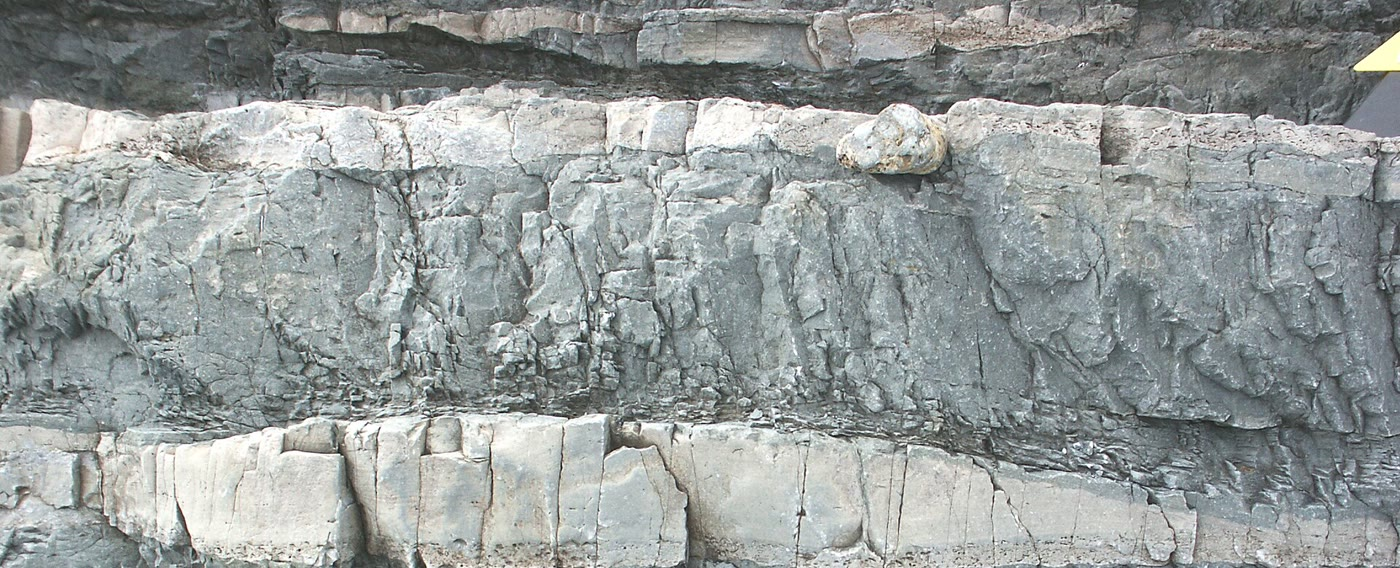
\includegraphics[width=\linewidth]{images/book5/b3-hummocky-cross-stratification.jpg}

{\scriptsize \omterm{def:b3:facies-models:hcs}{التطبّق المتقاطع الرابي} في تكوين أريسيغ
(السيلوري)، قرب أريسيغ، نوفا سكوشا. الصورة: \mbox{\textdir TLT Michael C. Rygel, CC BY-SA 3.0}
(مقصوصة).}
\end{minipage}
\end{inthefield}
% ledger: photo:b3-hcs

حيث يسود المدّ والجزر تتغيّر السحنات: تبني تيارات المدّ الصاعد والجزر
طبقاتٍ متقاطعةً تتجه في اتجاهين متعاكسين، وتترسّب غطاءات طينية عند كل
سكون المياه، وتتزايد سماكة الحُزم بين الغطاءات وتتناقص مع
دورة المدّ الربيعي والمدّ الميّت. وللقنوات المدّية والسهول المدّية وظهرات الرمل
نماذجها الخاصة، تُبنى بالطريقة نفسها.

\section{المياه العميقة}\label{sec:b3:facies-models:deep}

يُرسّب تيار العكرة الذي يتباطأ حمولته وفق ترتيب الترسيب:
أخشن الحبيبات أولًا وأدقّها أخيرًا. وتُظهر طبقة العكرة الكاملة هذا
الترتيب في خمسة أقسام.

\begin{definition}[متتالية بوما]\label{def:b3:facies-models:bouma}
\emph{متتالية بوما}\index{متتالية بوما} هي التعاقب المثالي للأقسام في
طبقة العكرة، من القاعدة إلى القمة: Ta، رمل كتيم أو مدرَّج على
قاعدةً تآكلية ذات علامات أخدودية وعلامات أدوات؛ Tb، رمل متوازي الرقائق؛ Tc،
رمل ناعم متقاطع الرقائق للتموّج الصغير وملتوٍ؛ Td، طمي متوازي الرقائق؛
Te، طين، جزء منه من تيار العكرة وجزء من الترسيب البطيء
بين التدفقات.
\end{definition}

قليلٌ من الطبقات يُظهر الأقسام الخمسة كلها: فقرب المصدر يكون التيار سريعًا ويترك
أقسامًا سميكةً من Ta تآكلت العليا منها بفعل التدفق التالي؛ وبعيدًا عنه لا يصل إلا
الأقسام الأدق، من Tc إلى Te. وتسجّل المتتالية بذلك
انحسار تدفّق واحد، ويسجّل تغيّر الطبقات على طول المروحة انحسار
التدفقات مع المسافة.

\begin{definition}[المروحة تحت البحرية]\label{def:b3:facies-models:fan}
\emph{المروحة تحت البحرية}\index{المروحة تحت البحرية} مخروط من الرواسب عند قاعدة
منحدر قارّي، تغذّيه وادٍ غائر: مروحة علوية ذات قناة رئيسية
تحدّها جسور طبيعية، ومروحة وسطى من القنوات المتفرعة تنتهي بفصوص رملية،
ومروحة سفلية من طبقات العكرة الرقيقة تنتقل إلى طين قاع الحوض.
\end{definition}

على طول الهامش، تعيد التيارات العميقة الناتجة عن دوران المحيط تشكيل
الرواسب الدقيقة للمنحدر إلى كونتورايت وتلالًا وركامات من
طمي وطين مُحرَّث بيولوجيًا ينمو على طول خطوط الكنتور لا إلى أسفل
المنحدر.

\begin{omfigure}
\begin{tikzpicture}[font=\scriptsize, x=1cm, y=1cm]
% (a) Bouma log
\begin{scope}
\fill[yellow!45] (0,0) -- (1.6,0) -- (1.6,1.2) -- (0,1.2) -- cycle;
\fill[yellow!35] (0,1.2) rectangle (1.3,1.8);
\fill[yellow!25] (0,1.8) rectangle (1.0,2.4);
\fill[black!12] (0,2.4) rectangle (0.7,2.8);
\fill[black!25] (0,2.8) rectangle (0.4,3.3);
\draw (0,0) -- (1.6,0) -- (1.6,1.2) -- (1.3,1.2) -- (1.3,1.8) -- (1.0,1.8) -- (1.0,2.4) -- (0.7,2.4) -- (0.7,2.8) -- (0.4,2.8) -- (0.4,3.3) -- (0,3.3) -- cycle;
\draw[decorate, decoration={snake, amplitude=0.5mm, segment length=2mm}] (0,0) -- (1.6,0);
\foreach \y in {1.35,1.5,1.65} {\draw[black!60] (0.05,\y) -- (1.25,\y);}
\foreach \x in {0.15,0.45,0.75} {\draw[black!60] (\x,1.95) .. controls (\x+0.08,2.1) .. (\x+0.2,1.95);}
\foreach \y in {2.5,2.6,2.7} {\draw[black!60] (0.05,\y) -- (0.65,\y);}
\foreach \y/\t in {0.6/Ta, 1.5/Tb, 2.1/Tc, 2.6/Td, 3.05/Te} {\node[anchor=west] at (1.9,\y) {\t};}
\node[anchor=west, align=left, font=\tiny] at (2.4,0.6) {\foreignlanguage{arabic}{رمل مدرَّج أو كتيم،}\\ قاعدة تآكلية};
\node[anchor=west, font=\tiny] at (2.4,1.5) {رقائق متوازية};
\node[anchor=west, font=\tiny] at (2.4,2.1) {تموّجات، رقائق ملتوية};
\node[anchor=west, font=\tiny] at (2.4,2.6) {طمي رقائقي};
\node[anchor=west, font=\tiny] at (2.4,3.05) {طين};
\node[anchor=north] at (1.6,-0.15) {\foreignlanguage{arabic}{(أ) طبقة عكرة}};
\end{scope}
% (b) fan plan
\begin{scope}[xshift=8.2cm, yshift=0.2cm]
\fill[black!8] (-1.0,-0.2) rectangle (5.6,3.1);
\fill[yellow!20] (0.3,2.9) .. controls (1.6,2.6) and (4.9,2.0) .. (5.2,0.9) .. controls (4.6,-0.1) and (1.2,0.1) .. (0.3,1.6) -- cycle;
\fill[yellow!45] (1.9,1.9) ellipse (0.55 and 0.3);
\fill[yellow!45] (2.6,1.0) ellipse (0.55 and 0.3);
\fill[yellow!45] (3.4,1.75) ellipse (0.5 and 0.28);
\draw[omDef, line width=1.4pt] (-0.9,3.0) .. controls (-0.3,2.8) and (0.4,2.6) .. (1.0,2.2);
\draw[omDef, line width=0.8pt] (1.0,2.2) -- (1.6,1.95);
\draw[omDef, line width=0.8pt] (1.0,2.2) -- (2.3,1.15);
\draw[omDef, line width=0.8pt] (1.0,2.2) .. controls (2.0,2.4) .. (3.1,1.85);
\node[anchor=south west] at (-0.95,3.0) {وادٍ غائر};
\node[anchor=east] at (0.55,2.0) {جسور طبيعية};
\node[align=center, font=\tiny] at (2.6,1.0) {فص};
\node at (4.4,0.7) {المروحة السفلية};
\node[black!60] at (4.9,2.85) {قاع الحوض};
\node[anchor=north] at (2.3,-0.25) {\foreignlanguage{arabic}{(ب) مروحة تحت بحرية في المسقط}};
\end{scope}
\end{tikzpicture}

\par\smallskip{\small (أ) \omterm{def:b3:facies-models:bouma}{متتالية بوما} لطبقة عكرة كاملة،
مرسومة كسجلّ لحجم الحبيبات (العرض يدلّ على خشونة أكبر)، مع أقسامها الخمسة. (ب)
\omterm{def:b3:facies-models:fan}{المروحة تحت البحرية} في المسقط: وادٍ غائر يغذّي قناةً بين جسور طبيعية، والتي
تتفرّع إلى قنوات توزيع تنتهي بفصوص رملية؛ وتنتشر عكراتٌ رقيقة
فوق المروحة السفلية.}\label{fig:b3:facies-models:deep}
\end{omfigure}

\section{المنصّات الكربوناتية}\label{sec:b3:facies-models:carbonates}

يتكوّن الرسوب الكربوناتي في موضعه، بفعل كائنات حية في مياه دافئة وصافية
ضحلة، وتتبع سحناته مقطع المنصّة التي يبنيها
المصنع الكربوناتي لنفسه.

\begin{definition}[المنحدر الكربوناتي والرصيف ذو الحافة]\label{def:b3:facies-models:ramp}
\emph{المنحدر الكربوناتي}\index{المنحدر الكربوناتي} هو منصّة يميل قاعها
بلطف وانتظام من خط الشاطئ نحو الحوض، دون انكسار:
أحزمتها السحنية، من السهول المدّية ورمال حواجز الشاطئ إلى حبيبات الضحاضح،
والرمل الفتاتي الحيوي والوحل الجيري البعيد عن الشاطئ، واسعةٌ وتنتقل تدريجيًا بعضها إلى بعض،
تفرزها طاقة الأمواج التي تتناقص مع العمق. أمّا \emph{الرصيف ذو
الحافة}\index{الرصيف ذو الحافة} فهو منصّة مسطّحة القمّة ذات انكسارٍ واضح في
الانحدار عند حافّتها، حيث تبني الشعاب والضحاضح الرملية حافةً تحمي بحيرةً خلفها؛
وخارج الحافة يُلقي منحدرٌ شديد الميل كتلًا وحبيبات في
الحوض.
\end{definition}

\begin{omfigure}
\begin{tikzpicture}[font=\scriptsize, x=1cm, y=1cm]
\begin{scope}
\fill[omSea!60] (0,1.6) -- (6.4,1.6) -- (6.4,0.3) -- cycle;
\fill[black!10] (0,1.6) -- (6.4,0.3) -- (6.4,0) -- (0,0) -- cycle;
\draw[thick] (0,1.7) -- (0.3,1.6) -- (6.4,0.3);
\draw[omDef] (0,1.6) -- (6.4,1.6);
\node[anchor=south] at (0.6,1.65) {السهول المدّية};
\node[rotate=-12, font=\tiny] at (1.5,1.08) {حبيبات الضحاضح};
\node[rotate=-12, font=\tiny] at (3.4,0.66) {الرمل الفتاتي الحيوي};
\node[rotate=-12, font=\tiny] at (5.3,0.26) {الوحل الجيري};
\node[anchor=north] at (3.2,-0.1) {\foreignlanguage{arabic}{(أ) المنحدر: ميل منتظم وأحزمة متدرّجة}};
\end{scope}
\begin{scope}[xshift=7.2cm]
\fill[omSea!60] (0,1.6) -- (6.4,1.6) -- (6.4,0.2) -- (4.4,0.3) -- (3.6,1.55) -- (3.2,1.6) -- (0.3,1.6) -- cycle;
\fill[omSea!60] (0.3,1.6) -- (3.2,1.6) -- (3.0,1.35) -- (0.6,1.35) -- cycle;
\fill[black!10] (0,1.7) -- (0.3,1.6) -- (0.6,1.35) -- (3.0,1.35) -- (3.2,1.6) -- (3.6,1.55) -- (4.4,0.3) -- (6.4,0.2) -- (6.4,0) -- (0,0) -- cycle;
\draw[thick] (0,1.7) -- (0.3,1.6) -- (0.6,1.35) -- (3.0,1.35) -- (3.2,1.6) -- (3.6,1.55) -- (4.4,0.3) -- (6.4,0.2);
\fill[orange!50] (3.05,1.4) -- (3.2,1.6) -- (3.55,1.56) -- (3.6,1.4) -- cycle;
\draw[omDef] (0,1.6) -- (6.4,1.6);
\node at (1.8,1.12) {البحيرة};
\node[anchor=south] at (3.35,1.65) {حافة الشعاب};
\node[anchor=west] at (4.2,0.95) {منحدر شديد};
\node at (5.5,0.6) {الحوض};
\node[anchor=north] at (3.2,-0.1) {\foreignlanguage{arabic}{(ب) رصيف ذو حافة: حافة، بحيرة، منحدر}};
\end{scope}
\end{tikzpicture}

\par\smallskip{\small مقاطع المنصّات الكربوناتية (تخطيطية، والمقياس الرأسي
مبالغ فيه كثيرًا). (أ) منحدر: أحزمة تفرزها طاقة الأمواج على طول
ميل منتظم. (ب) \omterm{def:b3:facies-models:ramp}{رصيف ذو حافة}: حافة من الشعاب والضحاضح عند انكسار الانحدار
تحمي بحيرةً من الوحل الجيري؛ ويتلقّى المنحدر الواقع خارجها كتلًا وحبيبات
المنفصلة عن الحافة.}\label{fig:b3:facies-models:platforms}
\end{omfigure}

على سطح منصّة مسطّح، يغمر ارتفاعٌ طفيف في مستوى البحر النسبي السهول المدّية،
ويعمل المصنع الكربوناتي بأسرع ما يكون في أضحل المياه، فيعيد ملء
الفراغ من جديد حتى مستوى سطح البحر في زمنٍ قصير. والنتيجة تتابعٌ من
الدورات شبه المدّية، بسماكة مترٍ أو بضعة أمتار، كلٌّ منها متتالية فرعية متناقصة العمق نحو الأعلى،
تمتدّ من وحل تحت المدّي إلى سهل مدّي تظهر فيه شقوق الجفاف أو
الحصائر الميكروبية، ويغطّيها \omterm{def:b3:sequence-stratigraphy:parasequence}{سطح الغمر} التالي.

\section{اللبّات وسجلّات الآبار}\label{sec:b3:facies-models:logs}

يُعرف معظم الصخور الواقعة تحت الأحواض الرسوبية من ثقوب الحفر. ويُؤخذ لبٌّ من عدد قليل منها،
وتوصف لبّاتها طبقةً طبقةً كما يُوصف الجرف؛ ويُسجَّل تقريبًا
جميعها.

\begin{definition}[سجلّات الآبار السلكية]\label{def:b3:facies-models:wireline}
\emph{سجلّ الآبار السلكي}\index{سجلّ الآبار السلكي} هو تسجيل متّصل لخاصية
فيزيائية للصخور بدلالة العمق، يُقاس بمسبار يُنزَل على
كابل إلى ثقب حفر. و\emph{سجلّ أشعة غاما}\index{سجلّ أشعة غاما} يسجّل
الإشعاع الغاميّ الطبيعي للصخر، بوحدات API: مرتفعًا في
الطَّفل، الذي يحتوي طينُه على البوتاسيوم والثوريوم واليورانيوم، ومنخفضًا في
رمال الكوارتز النقية والحجر الجيري. و\emph{سجلّ الكثافة}\index{سجلّ الكثافة} يسجّل
الكثافة الكلية من تشتّت أشعة غاما الصادرة عن
مصدرٍ مثبّت على المسبار. و\emph{السجلّ الصوتي}\index{السجلّ الصوتي} يسجّل
زمن العبور البيني لموجة ضغطية، بوحدة ميكروثانية لكل قدم.
و\emph{السجلّ النيوتروني}\index{السجلّ النيوتروني} يسجّل تباطؤ النيوترونات
بالهيدروجين، ومن ثمّ الماء المحتجَز في المسام وفي الطين.
\end{definition}
% ledger: keys:gamma, keys:density-porosity, keys:sonic

تُعرَّف وحدة أشعة غاما API في حفرة معايرة: جزءٌ من مئتين من
الفرق بين منطقة ذات نشاط إشعاعي مهمَل ومنطقة
تحتوي على النظائر المشعّة للطفل المتوسّط بتركيز يبلغ نحو ضعف تركيزه. والفحم،
والحجر الجيري والدولوميت عادةً أقلّ نشاطًا إشعاعيًا من الطَّفل؛ والحجر الرملي الكوارتزي منخفضٌ،
والأركوز الغنيّ بفلسبار البوتاسيوم أعلى؛ ويمكن لأيّ صخرٍ أن يصبح
مشعًّا بفعل اليورانيوم الذي تحمله المياه الجوفية.
% ledger: keys:gamma

\begin{proposition}[المسامية من الكثافة وزمن العبور]\label{prop:b3:facies-models:porosity}
صخرٌ مساميّته $\phi$، وكثافة حبيباته $\rho_{\mathrm{ma}}$
ومساماته مملوءة بسائل كثافته $\rho_f$، فيكون له الكثافة الكلية
$\rho_b = (1 - \phi)\rho_{\mathrm{ma}} + \phi\rho_f$، ومنه
\[
\phi = \frac{\rho_{\mathrm{ma}} - \rho_b}{\rho_{\mathrm{ma}} - \rho_f}.
\]
إذا عبرت موجة ضغطية الحبيبات والسائل على التوالي، بأطوال
متناسبة مع $1 - \phi$ و$\phi$، فيكون زمن عبورها
$\Delta t = (1 - \phi)\Delta t_{\mathrm{ma}} + \phi\Delta t_f$ (معادلة
المتوسّط الزمني)، و$\phi = (\Delta t - \Delta
t_{\mathrm{ma}})/(\Delta t_f - \Delta t_{\mathrm{ma}})$.
\end{proposition}

\begin{proof}
يحتوي وحدة حجم من الصخر على حجم $1 - \phi$ من الحبيبات و$\phi$ من
السائل، وكتلته $(1 - \phi)\rho_{\mathrm{ma}} + \phi\rho_f$، وهي
تُحلّ لإيجاد $\phi$. أمّا الموجة، فإنّ مسارًا طوله الوحدة يقطع $1 - \phi$ من
الحبيبات و$\phi$ من السائل، فتُجمع الأزمنة.
\end{proof}

كثافات الحبيبات \qty{2.65}{g/cm^3} للكوارتز، و\qty{2.71}{g/cm^3} في
الحجر الجيري؛ وماء المسام \qty{1.0}{g/cm^3} إن كان عذبًا، ويصل إلى
\qty{1.1}{g/cm^3} إن كان محلولًا ملحيًّا. وتتراوح أزمنة العبور من 42 إلى
\qty{48}{\micro\second/ft} في الدولوميت، ومن 48 إلى 53 في الحجر الجيري، و53 في
صخر رملي متماسك، و189 في المحلول الملحي. ومعادلة الكثافة دقيقةٌ من أجل
مصفوفة معلومة؛ أمّا معادلة المتوسّط الزمني فقاعدة تجريبية تعمل
أفضل ما يكون في الصخور المتماسكة ذات المسام البينحبيبية. ويخالف الطَّفل الاثنتين:
فللطين كثافاته الخاصة، ويحتجز ماءً مرتبطًا.
% ledger: keys:density-porosity, keys:sonic

\begin{definition}[نسبة الصافي إلى الإجمالي]\label{def:b3:facies-models:ntg}
\emph{نسبة الصافي إلى الإجمالي}\index{نسبة الصافي إلى الإجمالي} لفترة ما هي
سُمك صخرها ذي جودة الخزّان، وهو عادةً الرمل المُنتقى على \omterm{def:b3:facies-models:wireline}{سجلّ أشعة غاما}
تحت حدّ قطع، مقسومًا على السُّمك الكلّي للفترة.
\end{definition}

أداة سحنيّة لتحديد السحنة هي شكل منحنى أشعة غاما عبر جسم رملي.
\emph{الجرس}، وهو نظيف عند القاعدة ويزداد طفليةً نحو الأعلى، يمثّل
التعاقبَ المتناعم نحو الأعلى، كما في \omterm{def:b3:facies-models:rivers}{الحاجز النقطي} أو في ملء القناة؛ و\emph{القمعُ}، طفليّ عند
القاعدة ونظيف عند القمّة، وهو \omterm{def:b3:facies-models:association}{التعاقب المتخاشن نحو الأعلى}، كما في
\omterm{def:b3:facies-models:shoreface}{الوجه الشاطئي} المتقدّم أو جبهة الدلتا؛ و\emph{الأسطوانةُ}، نظيفة على امتدادها مع
حدود حادّة، تمثّل رملًا لنهر مضفور مُكدَّس أو كثيبًا ريحيًّا أو
حاجزًا كربوناتيًّا ضحلًا. والأشكال إشارات لا براهين: فيلزم أن يؤكّدها اللبّ،
أو على الأقل السجلّات المجاورة.

\begin{omfigure}
\begin{tikzpicture}
\begin{groupplot}[group style={group size=3 by 1, horizontal sep=0.2cm,
    y descriptions at=edge left},
  omrecord, y dir=reverse, ymin=700, ymax=1200, width=0.28\linewidth,
  height=0.62\linewidth, ytick={700,800,900,1000,1100,1200},
  tick label style={font=\scriptsize}, label style={font=\small},
  xlabel style={font=\small}]
\nextgroupplot[xlabel={\mbox{\textdir TLT GR (API)}}, ylabel={العمق \babelsublr{(\unit{m})}}, xmin=0, xmax=150,
  xtick={0,50,100,150}]
\addplot[black!60, densely dashed, forget plot] coordinates {(60,1046) (60,1166)};
% computed in figdata/bachelor-3/well_logs.py
\addplot[omDef, thin] table[x=gr, y=depth] {figdata/out/bachelor-3-well_logs-logs.dat};
\node[font=\scriptsize, anchor=west] at (axis cs:2,730) {الطباشير};
\node[font=\scriptsize, anchor=west] at (axis cs:2,816) {الطَّفل};
\node[font=\scriptsize, anchor=west] at (axis cs:28,956) {الحجر الجيري};
\node[font=\scriptsize, anchor=west] at (axis cs:28,1030) {الحجر الرملي};
\node[font=\scriptsize, anchor=west] at (axis cs:2,1185) {الشيست};
\nextgroupplot[xlabel={\mbox{\textdir TLT $\rho_b$ (\unit{g/cm^3})}}, xmin=1.9, xmax=2.9,
  xtick={2.0,2.4,2.8}, xticklabels={2.0,2.4,2.8}]
\addplot[red!70!black, thin] table[x=rhob, y=depth] {figdata/out/bachelor-3-well_logs-logs.dat};
\nextgroupplot[xlabel={\mbox{\textdir TLT $\Delta t$ (\unit{\micro\second/ft})}}, xmin=40, xmax=140,
  x dir=reverse, xtick={40,80,120}]
\addplot[green!40!black, thin] table[x=dt, y=depth] {figdata/out/bachelor-3-well_logs-logs.dat};
\end{groupplot}
\begin{axis}[at={(group c3r1.south east)}, xshift=1.35cm, anchor=south west,
  omrecord, y dir=reverse, ymin=1040, ymax=1172, width=0.28\linewidth,
  height=0.62\linewidth, xmin=0, xmax=120, xtick={0,60,120},
  ytick={1040,1060,1080,1100,1120,1140,1160}, ylabel={العمق \babelsublr{(\unit{m})}},
  xlabel={الحجر الرملي، \mbox{\textdir TLT GR (API)}}, tick label style={font=\scriptsize},
  label style={font=\small}]
\addplot[black!60, densely dashed, forget plot] coordinates {(60,1046) (60,1166)};
\addplot[omDef, semithick] table[x=gr, y=depth] {figdata/out/bachelor-3-well_logs-sand.dat};
\end{axis}
\end{tikzpicture}

\par\smallskip{\small سجلّات تركيبية لبئر فاردن-2 من \qty{700}{m}
إلى الركيزة: أشعة غاما (الخط المتقطّع هو حدّ القطع للرمل عند
\qty{60}{API} في الحجر الرملي)، والكثافة الحجمية وزمن العبور الصوتي (يتزايد الزمن نحو اليسار،
يتزايد نحو اليسار كما تُرسم السجلّات)؛ ويمينًا أشعة غاما للحجر الرملي
مكبَّرةً. تزداد كثافة الطباشير مع العمق؛
يُقرأ الطَّفل حارًّا وبطيئًا وذا كثافة متوسطة؛ والحجر الجيري بارد،
كثيفًا وسريعًا؛ والحجر الرملي مكدّسٌ من ملء القنوات، كلٌّ منها ذو قاعدة نظيفة
يتحوّل نحو الأعلى إلى طين: أشكال جرسية.}\label{fig:b3:facies-models:logs}
\end{omfigure}
% ledger: keys:gamma, keys:density-porosity, keys:sonic

\begin{inthelab}[تسجيل اللبّ]
\begin{minipage}[t]{0.5\linewidth}\vspace{0pt}
في مخزن اللُّبوب تُرصّ لُبوب البئر في صوانٍ، مشقوقةً طوليًّا،
مرتّبة حسب أعماقها. يصف عالِم الرسوبيات اللبّ
طبقةً طبقةً على ورقة السجلّ: حجم الحبيبات بعدسة يدوية وجدول المقارنة،
والبُنى والتماسّات والحفريات وآثار الجحور والجذور، ولونُ الطين.
ثم يُوضع الوصف بجانب سجلّات الآبار السلكية للأعماق نفسها،
وهذا يعاير أشكال السجلّات على الصخر ويتيح
قراءة الآبار المجاورة التي لم يُؤخذ لها لبّ.
\end{minipage}\hfill
\begin{minipage}[t]{0.46\linewidth}\vspace{0pt}
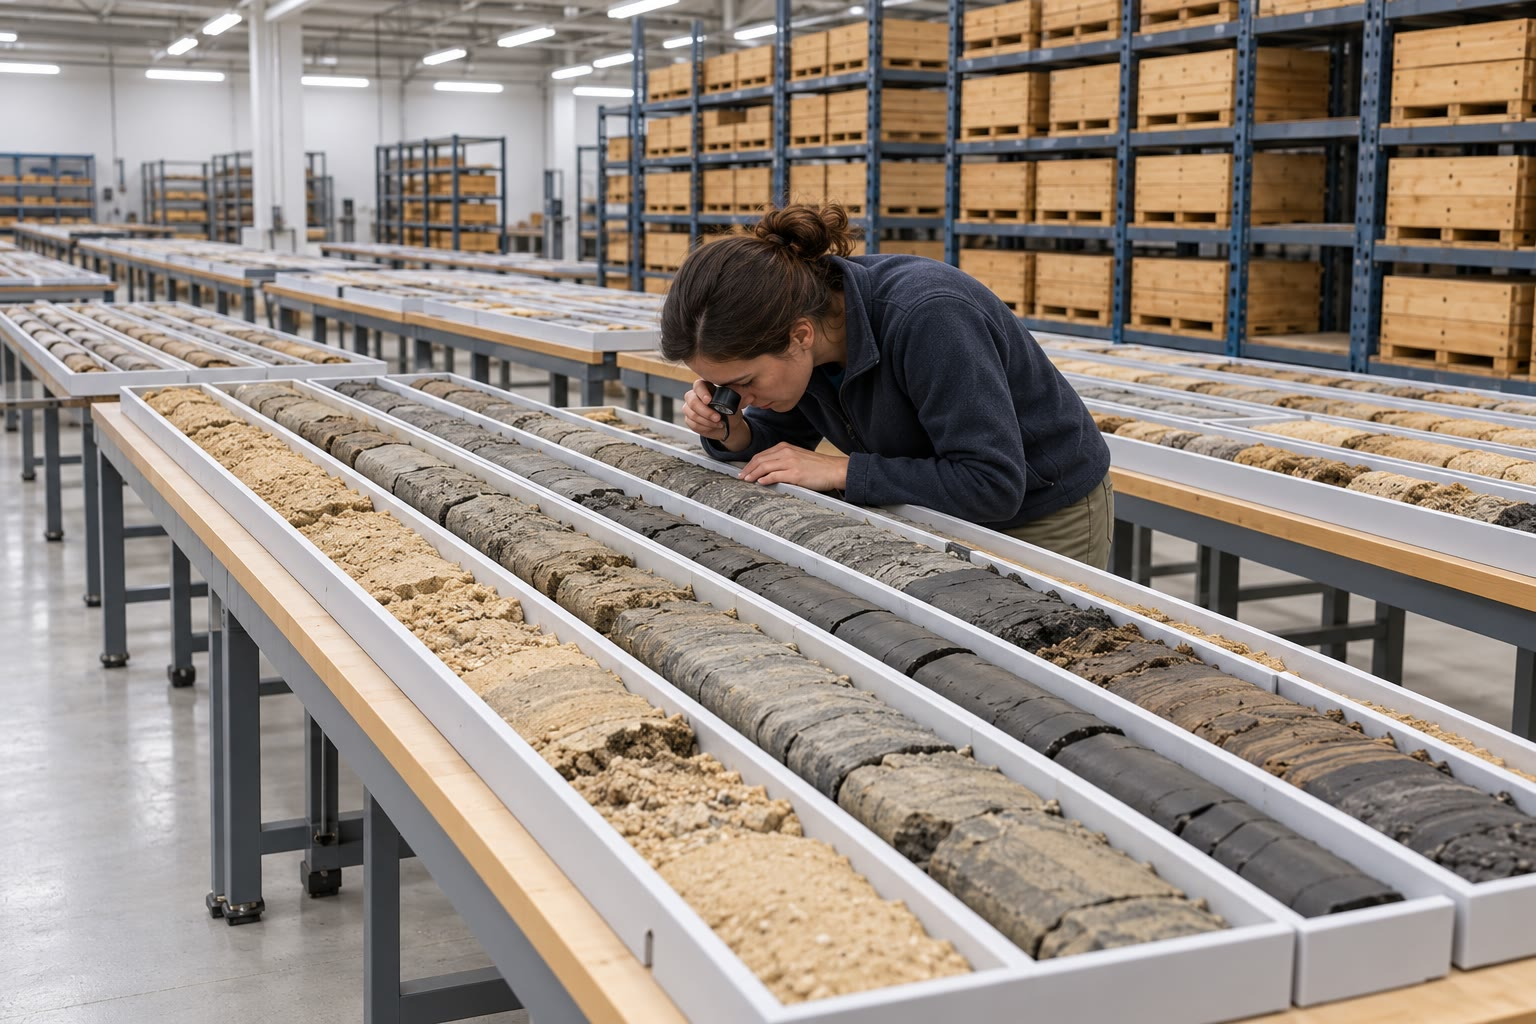
\includegraphics[width=\linewidth]{images/book5/ai/b3-core-store.jpg}

{\scriptsize مخزن اللُّبوب: لُبوب مشقوقة من الرمل والطين في صوانٍ، وعالم جيولوجيا
بعدسة يدوية. (رسم توضيحي مولَّد بالذكاء الاصطناعي).}
\end{minipage}
\end{inthelab}

\section{التمارين}

\begin{exercise}[$\star$]\label{exo:b3:facies-models:1}
يُظهر لبٌّ، من القاعدة نحو الأعلى: طينًا بعيدًا عن الشاطئ، وطينًا ورملًا ناعمًا متداخلَين،
ثم رملًا من \omterm{def:b3:facies-models:shoreface}{الوجه الشاطئي}، ورملًا شاطئيًّا، ثم فحمًا مع جذور. باستخدام قانون فالتر، حدِّد
ترتيب البيئات على طول الساحل في ذلك الزمن، والاتجاه
الذي تحرّك فيه خطّ الشاطئ. ماذا كان سيُخلّف التجاوز البحري؟
\end{exercise}

\begin{exercise}[$\star$]\label{exo:b3:facies-models:2}
تُظهر ثلاثة أجسام رملية أشكالًا لأشعة غاما: (أ) جرسًا سُمكه \qty{8}{m} وذا
قاعدةً حادّة؛ (ب) قمعًا سُمكه \qty{20}{m}؛ (ج) أسطوانةً سُمكها
\qty{30}{m} ذات قمّة وقاعدة حادّتين. اقترح بيئةً لكلٍّ منها، والملاحظةَ
في اللبّ التي من شأنها أن تؤكّدها.
\end{exercise}

\begin{exercise}[$\star$]\label{exo:b3:facies-models:3}
يُقرأ صخر رملي $\rho_b = \qty{2.40}{g/cm^3}$. احسب مساميته بمصفوفة كوارتزية وماء عذب،
ثم بمحلول ملحي كثافته \qty{1.1}{g/cm^3}.
\end{exercise}
% ledger: keys:density-porosity

\begin{exercise}[$\star$]\label{exo:b3:facies-models:4}
أمواج طول موجتها المنوالي \qty{75}{m} و\qty{110}{m} (البحر المحمي والبحر المفتوح
في دراسة العوامة). قدّر العمق الذي تحتفظ عنده كلٌّ منها بنسبة
\qty{4}{\percent} من حركتها السطحية، والكسر المتبقّي عند عمق
\qty{20}{m}.
\end{exercise}
% ledger: losspeters10:wavebase

\begin{exercise}[$\star\star$]\label{exo:b3:facies-models:5}
يُقرأ حجر جيري $\Delta t = \qty{60}{\micro\second/ft}$. احسب مساميته
بمعادلة المتوسط الزمني لمصفوفة قيمتها 47.6
و\qty{52.6}{\micro\second/ft} ولمحلول ملحي عند \qty{189}{\micro\second/ft}. ماذا
يعلّمنا الفرق؟
\end{exercise}
% ledger: keys:sonic

\begin{exercise}[$\star\star$]\label{exo:b3:facies-models:6}
فترة سُمكها \qty{40}{m} تحوي طبقات رملية سُمكها 6.0، 3.5، 8.0 و\qty{2.5}{m}
تحت حدّ القطع، والباقي طينًا. احسب \omterm{def:b3:facies-models:ntg}{نسبة الصافي إلى الإجمالي}. بمسامية
\qty{22}{\percent} في الرمل، ما حجم المسام الذي تحويه
كيلومترًا مربعًا من الفترة؟
\end{exercise}

\begin{exercise}[$\star\star$]\label{exo:b3:facies-models:7}
طبقة عكرة قرب مصبّ وادٍ سحيق سُمكها \qty{1.2}{m} من رمل كتليّ
\babelsublr{(Ta)} تآكلت قمّتها بفعل الطبقة التالية؛ وعلى بُعد \qty{30}{km} أسفل المروحة، طبقة
من التيّار نفسه هي \qty{8}{cm} من رمل ناعم وطمي ذي تطبّق متموّج، تحت
\qty{3}{cm} من الطين. سمِّ أقسام كلٍّ منهما وفسّر التغيّر.
\end{exercise}

\begin{exercise}[$\star\star$]\label{exo:b3:facies-models:8}
\omterm{def:b3:facies-models:association}{التعاقب المتناعم نحو الأعلى} سُمكه \qty{9}{m} له قاعدة حادّة مع حصى،
ورمل متصالب الطبقات، ورمل ناعم متموّج، وطين ذو جذور. فسِّره، وقدِّر
عمق القناة التي كوّنته. هل يمكن تطبيق قانون فالتر عبر قاعدته؟
ولماذا؟
\end{exercise}

\begin{exercise}[$\star\star$]\label{exo:b3:facies-models:9}
ينخفض قاع منصّة بمقدار \qty{60}{m} على امتداد \qty{40}{km}؛ ومنصّة أخرى
تحافظ على عمق \qty{5}{m} لمسافة \qty{30}{km}، ثم تنخفض \qty{300}{m} على
امتداد \qty{1.5}{km}. احسب الانحدارين، وسمِّ كلّ منصّة والسحنة
المتوقّعة عند حافة الثانية.
\end{exercise}

\begin{exercise}[$\star\star\star$]\label{exo:b3:facies-models:10}
يتقدّم خطّ الشاطئ بسرعة $v$ بينما يرتفع مستوى البحر النسبي بمعدّل
$A$، وحزامه الشاطئي عرضه $w$. بيّن أنّ رمل \omterm{def:b3:facies-models:shoreface}{الوجه الشاطئي} في التعاقب
الرأسي سُمكه $h = wA/v$. احسب ذلك من أجل $w = \qty{2}{km}$،
$A = \qty{0.2}{m/kyr}$ و$v = \qty{20}{m/kyr}$، وبيّن ماذا يحدث عندما
$A = 0$. قارن بالقضية المتعلقة \omterm{def:b3:sequence-stratigraphy:trajectory}{بمسار خط الشاطئ} في
الفصل~\ref{ch:b3:sequence-stratigraphy}.
\end{exercise}

\begin{exercise}[$\star\star\star$]\label{exo:b3:facies-models:11}
يُقرأ صخر رملي $\rho_b = \qty{2.30}{g/cm^3}$ و$\Delta t =
\qty{86}{\micro\second/ft}$. احسب مساميته من كلّ سجلّ بمصفوفة من الحجر الرملي الكوارتزي
(كثافتها 2.65، وزمن عبورها \qty{52.6}{\micro\second/ft}) وبمحلول ملحي (كثافته 1.0،
وزمن عبوره \qty{189}{\micro\second/ft}). إن كانت المسامية الصوتية صحيحة، فما
كثافة الحبيبات التي يقتضيها \omterm{def:b3:facies-models:wireline}{سجلّ الكثافة}، وما الذي قد يكون عليه الإسمنت؟
\end{exercise}
% ledger: keys:density-porosity, keys:sonic

\begin{exercise}[$\star\star\star$]\label{exo:b3:facies-models:12}
في اللبّ، يرقد طين بحري أسود مباشرةً فوق فحم ذي جذور، مع طبقة رقيقة
من فتات الأصداف عند التماس. فسِّر لماذا لا ينطبق قانون فالتر عبره، وما هو هذا السطح،
وكم من التعاقب الساحلي قد يكون مفقودًا
إذا تآكلت الأمواج القاع حتى \omterm{def:b3:facies-models:shoreface}{قاعدة أمواج الطقس الهادئ} البالغة نحو \qty{10}{m}
أثناء مرور خطّ الشاطئ.
\end{exercise}

\section{مسألة: فاردن-2، بئر تخترق الغطاء}

\begin{problem}[{مسألة نهاية الأسبوع --- السجلّات والمسامية والسحنات والرمل الصافي
لبئر مُختلقة في الطية المقعرة لتلال فاردن}]
\label{pb:b3:facies-models:1}
تُحفر البئر فاردن-2 في الطية المقعرة لتلال فاردن، عند الإحداثيات \babelsublr{(7500, 7000)} على
شبكة الإقليم، وتبدأ من منسوب أرضي قدره \qty{441.0}{m}،
وتبلغ عمقًا كليًّا قدره \qty{1200}{m}. وتُرسم سجلّاتها في شكل القسم الأخير.
استخدم كثافات حبيبات قدرها 2.65 (للكوارتز)
و\qty{2.71}{g/cm^3} (للكالسيت)، وماء مسامٍ كثافته \qty{1.0}{g/cm^3}، وأزمنة عبور المصفوفة
52.6 (للحجر الرملي) و\qty{47.6}{\micro\second/ft}
(للحجر الجيري)، و\qty{189}{\micro\second/ft} للماء.

\medskip\noindent\textbf{الجزء الأول --- قراءة السجلّات.}
\begin{enumerate}
\item تقفز أشعة غاما من 12 إلى \qty{110}{API} عند \qty{766}{m}، ثم تنخفض
  إلى 18 عند \qty{866}{m}، وتصبح غير منتظمة من \qty{1046}{m} وتستقرّ عند
  \qty{85}{API} من \qty{1166}{m}. سمِّ الوحدات التي صادفتها، مستعينًا بسجلّاتها.
\item احسب سُمك كلّ وحدة من وحدات الغطاء ومنسوب
  قاعدة الغطاء.
\item تبلغ كثافة الطباشير \qty{2.03}{g/cm^3} قرب السطح،
  و\qty{2.36}{g/cm^3} عند \qty{750}{m}. احسب مساميته عند العمقين.
  ماذا يحدث للطباشير مع العمق؟
\item لماذا لا تُحسب مسامية الطَّفل من كثافته؟
\item يُقرأ الشيست \qty{2.75}{g/cm^3} و\qty{50}{\micro\second/ft}.
  ماذا يخبر الحفّارَ الأساسُ الصخريّ السريع الكثيف عديم المسامية؟
\end{enumerate}

\medskip\noindent\textbf{الجزء الثاني --- المسامية.}
\begin{enumerate}[resume]
\item يُقرأ الحجر الجيري \qty{2.573}{g/cm^3}: احسب مساميته بطريقة الكثافة.
\item يُقرأ الحجر الجيري نفسه \qty{58.9}{\micro\second/ft}: احسب مساميته الصوتية
  وقارن بين النتيجتين.
\item يُقرأ الرمل النقي في ملء القناة \qty{2.32}{g/cm^3}: احسب
  مساميته.
\item تحقّق منها بزمن عبورها \qty{79.9}{\micro\second/ft}.
\item لو كان ماء المسام محلولًا ملحيًّا كثافته \qty{1.1}{g/cm^3}، فبمقدار كم
  ستتغيّر مسامية الكثافة للرمل؟
\item أيّ الوحدتين تكون الأفضل خزانًا جوفيًّا أو مكمنًا، وأيّهما
  الحاجز الذي يعلوها؟
\end{enumerate}

\medskip\noindent\textbf{الجزء الثالث --- السحنات.} اللبّ المأخوذ من 1108 إلى
\qty{1124}{m} يُظهر من القاعدة: سطحًا محتتًّا مع فتات طينية
وحصًى؛ \qty{10.4}{m} من رمل متوسط متصالب الطبقات؛ \qty{3.2}{m} من رمل
ناعم متموّج يتدرّج إلى طمي؛ \qty{2.4}{m} من طين بنّي مائل إلى الحمرة مع آثار جذور.
\begin{enumerate}[resume]
\item ارسم شكل \omterm{def:b3:facies-models:wireline}{سجلّ أشعة غاما} المتوقّع عبر الفترة المأخوذ لبّها.
\item سمِّ التعاقب وبيئة كل جزء.
\item بالاستعانة بقانون فالتر، صِف البيئات التي كانت تقع جنبًا إلى جنب.
\item قدِّر عمق القناة.
\item يحوي الحجر الرملي أحد عشر وحدةً من هذا النوع، كلٌّ منها على قاعدة حادّة. ماذا
  يُخبر التراكب عن النهر وسهله الفيضي؟
\item هل يصلح قانون فالتر للانتقال من وحدة إلى التي تليها؟ لماذا؟
\end{enumerate}

\medskip\noindent\textbf{الجزء الرابع --- الرمل الصافي.} ملءات القنوات الأحد عشر،
من قاعدة الحجر الرملي هي 14، 9، 12، 7، 16، 10، 13، 8، 11، 12
و\qty{8}{m} سمكًا. تبدأ كل منها برمل نظيف بقيمة \qty{30}{API} يشغل نسبةً
من سمكها: 0.60، 0.45، 0.55، 0.30، 0.65، 0.40، 0.55، 0.35، 0.50،
0.45 و0.30، ثم يتناعم نحو الأعلى على نسبة 0.25، 0.30، 0.25، 0.40،
0.20، 0.30، 0.25، 0.35، 0.25، 0.30 و0.35، ترتفع أشعة غاما خطيًّا حتى
\qty{105}{API}، وتنتهي بالطين.
\begin{enumerate}[resume]
\item ما الكسر من كل فترة تناعم الواقع أسفل
  حدّ القطع \qty{60}{API}؟
\item احسب الرمل الصافي للوحدة السفلى وللوحدة الأسمك.
\item احسب مجموع الرمل النظيف ومجموع فترات التناعم في
  الحجر الرملي.
\item احسب \omterm{def:b3:facies-models:ntg}{نسبة الصافي إلى الإجمالي} له.
\item كيف يتغيّر الرمل الصافي إذا كان حدّ القطع 45 أو
  \qty{75}{API}؟
\item بمسامية الرمل الواردة في السؤال 8، احسب حجم المسام في
  الرمل الصافي تحت كيلومتر مربّع واحد.
\item اذكر سُمك الرمل الصافي للحجر الرملي الترياسي عند فاردن-2.
\end{enumerate}
\end{problem}
% ledger: keys:density-porosity, keys:sonic, keys:gamma
